

\chapter{IP3 and IP3-gated ion channels}
\label{chap:ip3-gated-ion}


{\it IP3-gated ion channels} (or IP3 receptors, IP3R) is a type of
\ce{Ca^2+}-channel whose activation is mediated by IP3. Thus, IP3-gated ion
channels is also called {\it IP3-receptors} (IP3Rs). 

IP3Rs are often found in nonmuscle cells (e.g. nerve cells), but also in cardiac
cells (Sect.\ref{sec:IP3R_cardiac}). In this chapter, we first examine the
structure of IP3, IP3R and its isoforms, then the IP3-signaling pathways.

% There is no longer any
% doubt that IP3 plays crucial physiological and pathological role in the heart.
% These roles, however, are incompletely understood and remain to be defined more
% precisely. 

\section{Introduction}

\subsection{Inositol (myo-inositol)}
\label{sec:inositol}
\label{sec:myo-inositol}

% The first component of IP3 is {\it myo-inositol} - a prominent 3D structure of
% inositol. 

{\bf Inositol} (cyclohexane 1,2,3,4,5,6-hexol) is a 6-fold alcohol of
cyclohexane. Inositol has 9 possible {\it steroisomers} (Sect.\ref{sec:isomer})
with the prominent form is cis-1,2,3,5-trans-4,6-cyclohexanehexol, aka {\it
myo-inositol} (mI), as shown in Fig.~\ref{fig:inositol}. 

\textcolor{red}{Myo-inositol is the first component of IP3}
(Sect.\ref{sec:IP3}), and the structural lipid phosphatidylinositol
(Sect.\ref{sec:phosphatidylinositol}).
Myo-inositol's three dimensional structure looks
like a chair. It has a ring of 6 carbons. The carbons are numbered in an
anticlockwise direction when the ring is viewed from above.

{\bf NOTES}: Myo-inositol is found in many food, cereal, nuts, beans,
and fruits, especially melons and oranges.

  \begin{figure}[htb]
    \centerline{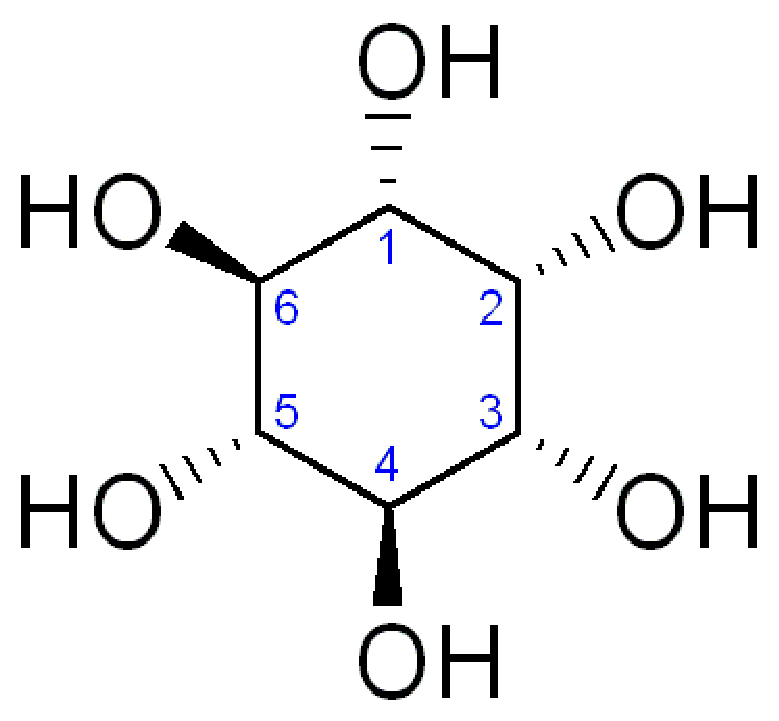
\includegraphics[height=3cm]{./images/inositol_structure.eps},
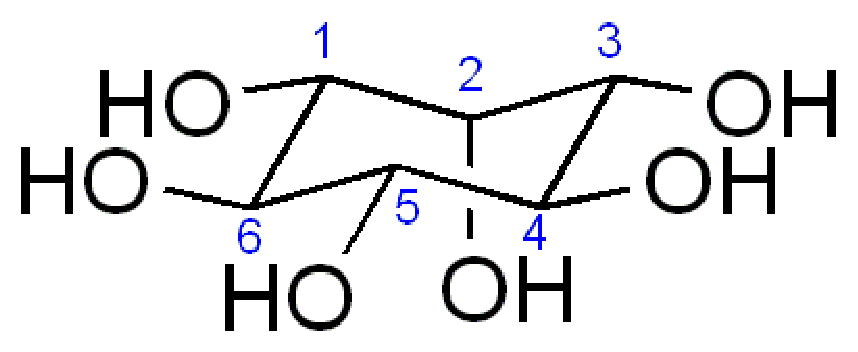
\includegraphics[height=2cm]{./images/inositol_chair.eps}}
\caption{Myo-inositol
  (cis-1,2,3,5-trans-4,6-cyclohexanehexol), where the
  hydroxyl groups (-OH) are on the same side at position
  1,2,3,5}\label{fig:inositol}
  \end{figure}

As shown in Fig. \ref{fig:agranoff}, myo-inositol has a plane of symmetry
running through carbon atoms 2 and 5 which divides the molecule into chiral
halves, i.e. each half mirroring to each other through the plan crossing carbons
2 and 5.  Thus, any substitution on carbon 1,3,4 or 6 will alter this symmetry
and the product be designated as D- or L- form (Sect.\ref{sec:D-and-L-form}). 
However, as L-form and D-form are exchangeable, \textcolor{red}{UIPAC
nomenclature suggests to use D-form for myo-inositol}.
Agranoff's turtle is a useful mnemonic for remembering inositol phosphates
numbering, as shown in Fig.~\ref{fig:agranoff}.

\begin{figure}[htb]
  \centerline{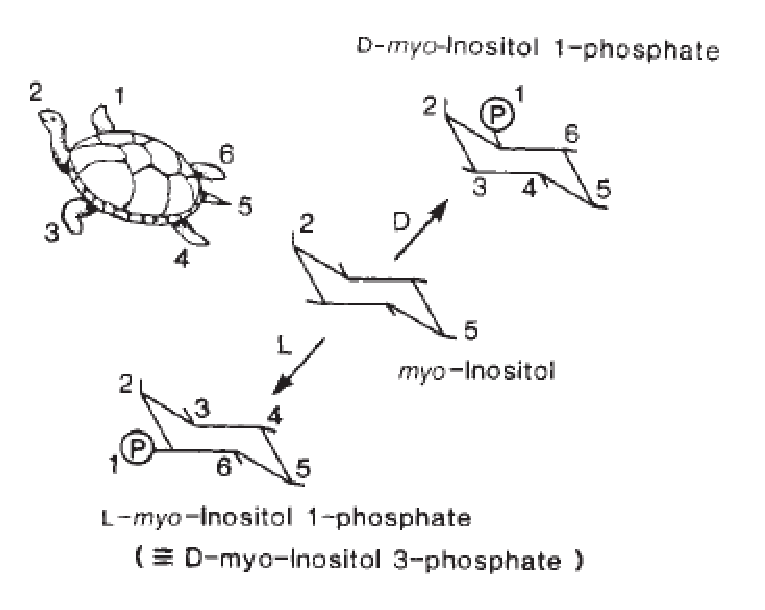
\includegraphics[height=6cm]{./images/agranoff_turtle.eps}}
  \caption{Agranoff's turtle}\label{fig:agranoff}
\end{figure}

Myo-inositol plays at least two important physiological roles in the central
nervous system (CNS)
\begin{enumerate}
  
  \item cell osmotic regulation (Nakinishi
et al., 1989)
  
  \item phosphoinositide signal transduction pathway (Berridge
and Irvine, 1989).
\end{enumerate}

Some studies confirmed that myo-inositol (mI), an osmolyte, is exclusively glial
and based on these results, myo-inositol has been suggested for use as a
glia-specific marker for in vivo MRS studies (Brand, Richter- Landsberg,
Leibfritz, 1993).
However, Moore et al. (1999) suggested that it is not exclusively glial cells,
at least in human CNS. Further reading is required to get more data for
conclusion. Read Sect.\ref{chap:neuro-marker} for information about neuro
markers.


\subsection{Inositol phosphate}
\label{sec:inositol-phosphate}

The six carbons (each with 1 hydroxyl group) that comprise the inositol ring
(Sect.\ref{sec:inositol}) can be phosphorylated in a combinatorial manner,
generating a truly astonishing range of {\bf inositol phosphates} and inositol
lipids. \textcolor{red}{The order of attaching phosphate groups to myo-inositol
is following the given orders: 4, 1, 5, 3.} 

\begin{itemize}
\item D-myo-inositol 4-monophosphate
\item D-myo-inositol 1,4-biphosphate
\item D-myo-inositol 1,4,5-triphosphate (Ins(4,1,5)P$_3$)

\textcolor{red}{IP3 (Sect.\ref{sec:IP3}) is {\bf D-myo-inositol
1,4,5-triphosphate}}.

\item D-myo-inositol 1,3,4,5-tetrakphosphate
\item D-myo-inositol pentakisphosphate
\item D-myo-inositol hexakisphosphate

{\bf NOTE}: There is no order with pentakisphosphate and
hexakisphosphate~\citep{berridge1989ipa}.
\end{itemize}


\section{IP3 (D-myo-inositol 1,4,5-triphosphate)}
\label{sec:IP3}
\label{sec:IP3_structure}

IP3 is the phosphorylated form of D-myo-inositol (Sect.\ref{sec:inositol}) at 3
locations, giving its the name D-myo-inositol 1,4,5-triphosphate.
In the previous chapter, we have mentioned \ce{Ca^2+} as one of the
second-messenger agents. Now we come to introducing another second messenger
agent, {\bf inositol-1,4,5-triphosphate} (Ins(1,4,5)P3 or IP3) or precisely as
{\bf D-myo-inositol 1,4,5-triphosphate}. The role of IP3 as the second
messenger, and the upstream of calcium release from ER is discussed in
Sect.\ref{sec:PLC-Calcium}.

Like calcium, IP3 is a second-messenger that involves in many intracellular
signalling (Sect.\ref{sec:ip3-pathways}).



\section{IP3 signal transduction pathways}
\label{sec:ip3-pathways}
%\section{IP3 and IP3R functions}

{\bf SUMMARY}: This signal transduction involves 3 main components:
a receptor, a coupling G protein and a PLC-$\beta$. In many types of eukaryotic
cells, the suggested mechanism is that the specific receptor when bound by a
ligand, will activate the trimeric G protein. The alpha subunit of this
activated G protein then (G$\alpha$q/11) activates phospholipase C (aka
phosphoinositidase C). As told by its name, phospholipase C cleaves off IP3 from
the plasma membrane, with DAG as the other product. Then IP3 can diffuse into
the cytoplasm. IP3 raises the cytosolic level of calcium ion by releasing it from
the endoplasmic reticulum (Sect.\ref{sec:GPCR-PLC-IP3-DAG-pathway}).

% In many types of eukaryotic cells, the suggested mechanism is that the
% activation of surface receptors leads to the production of
% inositol-1,4,5-trisphosphate (IP3). Receptor-activated phospholipase C generate
% IP3 and DAG. IP3 raises the cytosolic level of calcium ion by releasing it from
% the endoplasmic reticulum (Sect.\ref{sec:GPCR-PLC-IP3-DAG-pathway}).

\IPthree has been shown to mobilize free $\Ca$ (from resting level 0.2$\muM$ to
0.6$\muM$), and causing discrete spikes \citep{meyer1991} or a series of $\Ca$
transients rising periodically (i.e. oscillation) \citep{woods1987, dupont2000}.
A dedicated chapter for calcium wave from IP3 is given in
Chap.\ref{chap:calcium_waves_IP3R}.

At low $[\Ca]_i$, IP3-bound receptor is unlikely to open. When spontaneous
openings of IP3R do occurs, it triggering the release of $\Ca$ from
intracellular stores \citep{berridge1993}. The nearest neighbor IP3-bound
receptor is on average too far away for the released $\Ca$ to diffuse to it.
However, when $[\Ca]_i$ is high, it increase the opening probability $P_o$ of
the IP3-bound receptors, bringing more $\Ca$ to be released. This feedback takes
place between IP3-R that are less than 1$\mum$ apart, and the feedback effect of
$\Ca$ occur within 2ms after being released \citep{wang1993lpf}.

\begin{framed}
The average distance between IP3 receptors of 0.3 $\mum$
if the IP3 receptor has one binding site for IP3, and 0.5 $\mum$
if it has four.

\end{framed}


These two processes (Ca2+ influx via VSCC, and Ca2+ release from ER) have been
known to be linked in some way long before the nature of that linkage was known
(Putney, 1977). Upon production (Sect.\ref{sec:IP3_synthesis}), \IPthree
diffuses rapidly into the cell interior to perform its signaling function.
\begin{enumerate}

  \item  The first report on the second messenger role of IP3 - and also is
  commonly used nowadays - was its binding to the receptor - \tIPthreeR - the
  gating of $\Ca$ \citep{berridge1993,  streb1983rcn}. IP3 induces the release
  of \ce{Ca^2+} from non-mitochondrial internal stores, mainly ER/SR, which can
  link to calcium oscillation (Sect.\ref{sec:IP3-calcium-oscillation}). However,
  IP3 has also been shown to release \ce{Ca^2+} from other compartments (as
  microdomains), e.g. Golgi, nuclear envelope\citep{rizzuto2006mic}. 

The released $\Ca$ then provide a positive feedback to trigger further $\Ca$
release by activating RyR and IP3R from the cytosolic side. This requires IP3R
to be near RyR2. However, the subcellular distribution of both IP3R and RyR2 are
still under investigating.


   \item 

\end{enumerate}


\begin{figure}[hbt]
 \centerline{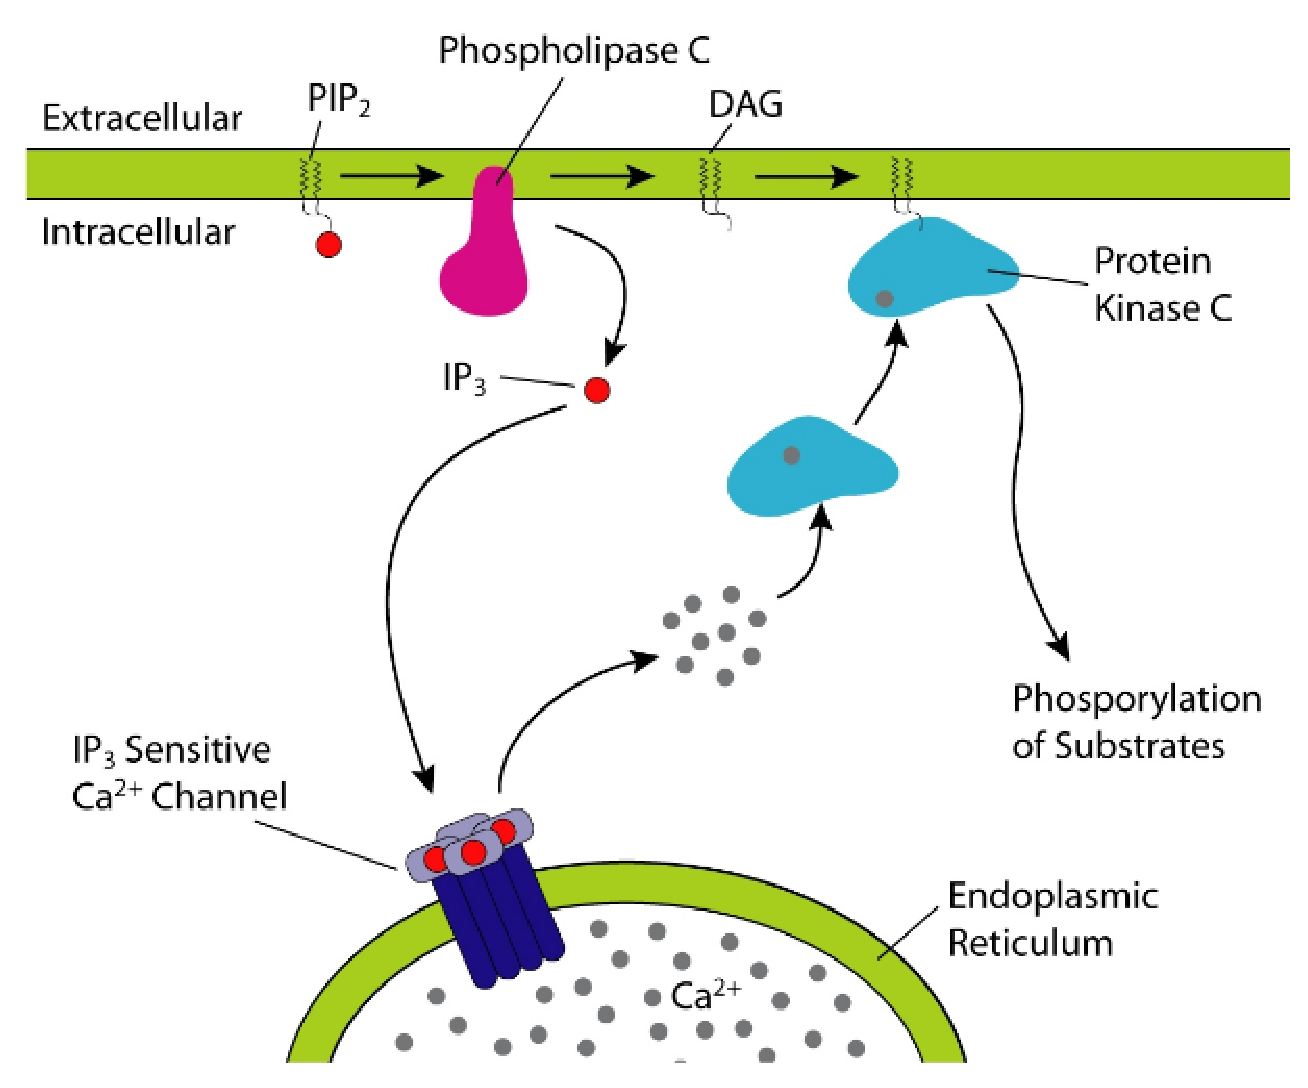
\includegraphics[height=7cm]{./images/IP3_DAG_pathway.eps}}
\caption{IP3/DAG pathways}
\label{fig:IP3-DAG}
\end{figure}



IP3 rapidly diffuses and binds to the InsP3-receptor Ca2+ channels in the ER
membrane, inducing Ca2+ release. IP3Rs are specific to calcium only, as shown in
Fig.~\ref{fig:IP3-IP3R}.  It's only IP3 synthesized from $G_{\alpha
q/11}$ can bind to IP3R (Sect.\ref{sec:IP3R}).
\begin{enumerate}
  \item cardiac myocyte - Sect.\ref{sec:IP3R_cardiac}
  
  \item neuron - Sect.\ref{sec:IP3R_neuron}
\end{enumerate}

The increase in concentration of IP3 allows IP3 to bind to IP3-receptors, and
induces the release of \ce{Ca^2+} from internal stores ER or, indirectly, by
stimulating calcium entry~\citep{berridge1989ipa}. $\Ca$ release can display
different patterns (Sect.\ref{sec:IP3-calcium-oscillation}). This suggest that
the potential role of IP3 go beyond the release of \ce{Ca^2+} from internal
store\citep{kockskamper2008ip3}.


\begin{figure}[hbt]
 \centerline{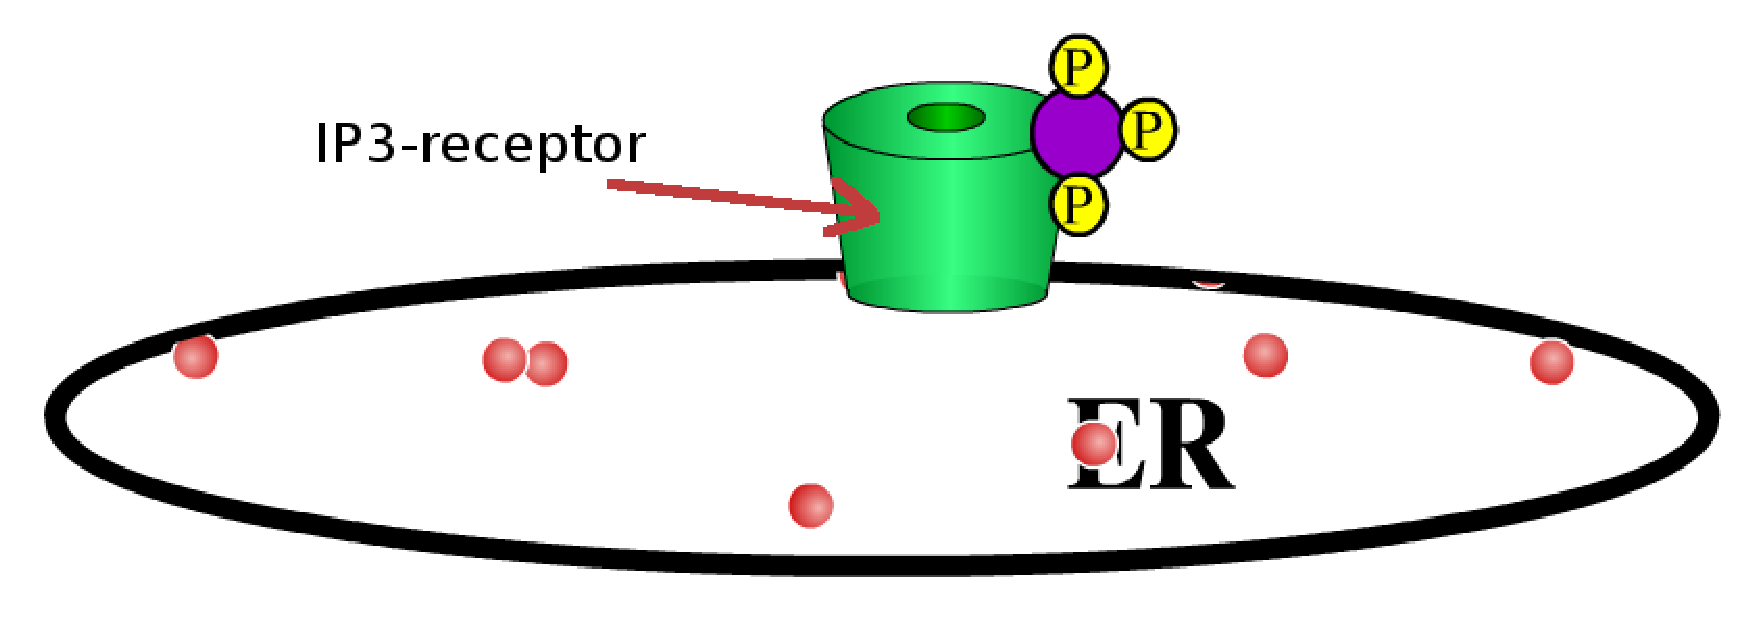
\includegraphics[height=3cm]{./images/IP3_bind_IP3R.eps}}
\caption{IP3 bind to IP3-receptors to trigger the release of
  \ce{Ca^2+} from SR}
\label{fig:IP3-IP3R}
\end{figure}


  \begin{figure}[htb]
    \centerline{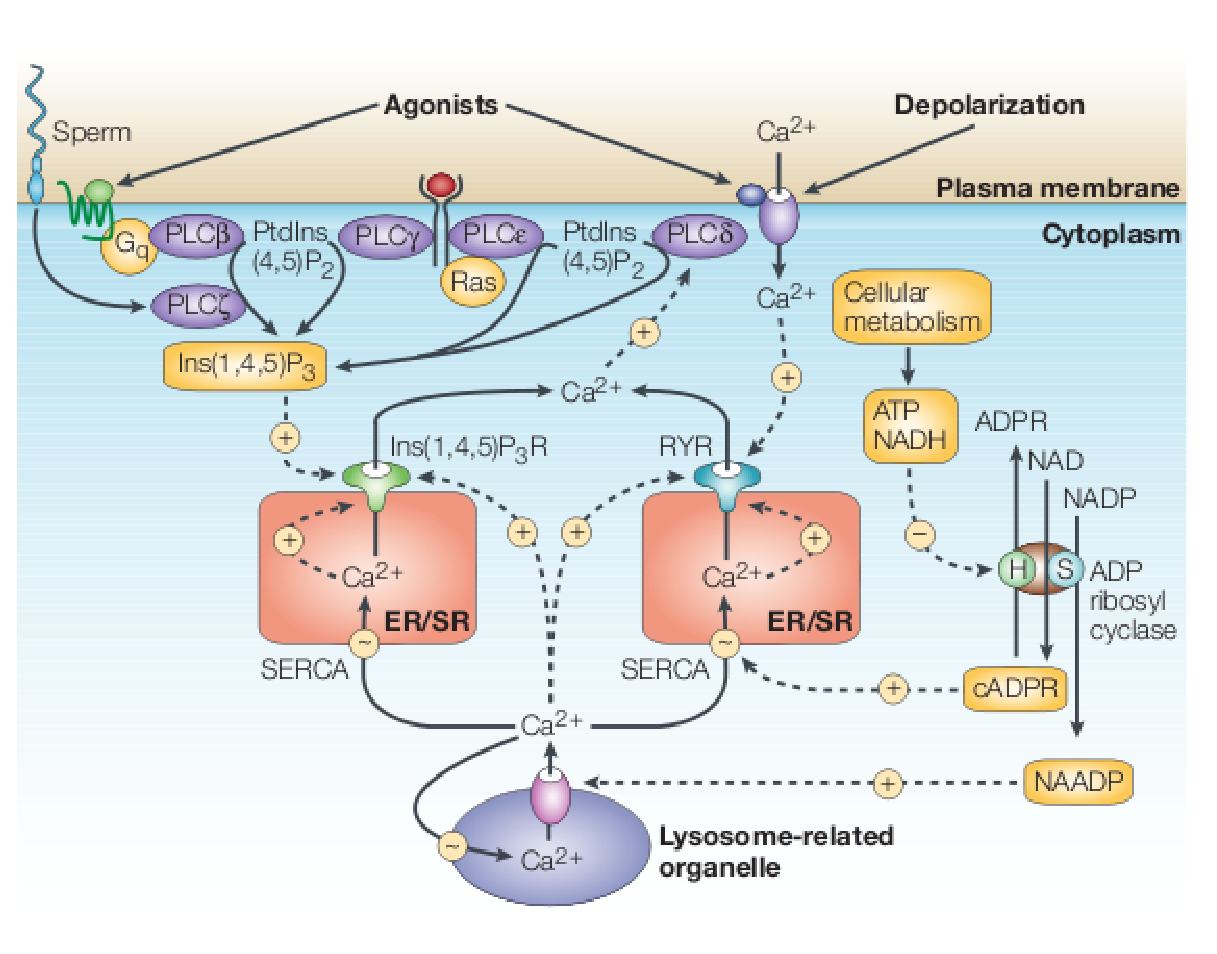
\includegraphics[height=8cm]{./images/calcium_mobilizing.eps}}
    \caption{Calcium-mobilizing messengers and modulators}\label{fig:Ca_mobilizing}
  \end{figure}

Another product in the production of IP3 is PKC (Sect.\ref{sec:PKC}), which may
inhibit IP3 production by inactivating agonist receptors.
However, it is not known whether the involvement of these Ca21-dependent
feedback mechanisms serves a physiological role.

% However, IP3 is \textcolor{red}{unlikely} to be a key player in
% cardiac excitation-contraction (EC) coupling, but RyR receptors in a
% process known as CICR.

% The release of IP3 into the cytoplasm mobilizes \ce{Ca^2+} from
% non-mitochondrial internal storage which is believed to be ER/SR. 

% TECHNICAL TERMS:
% receptor-operated channel = ligand-binded channel = second
% messenger-operated channel

% voltage-gated channel

\subsection{Synthesis IP3: PLC $\rightarrow$ IP3 +
DAG}
\label{sec:IP3_synthesis}
\label{sec:IP3-production}

% At the biomembrane, there is a type of transmembrane {\it receptor proteins},
% called {\bf G proteins-coupled receptor} (GPCR - Sect.\ref{sec:GPCR}), as
% shown in Fig.~\ref{fig:IP3}.

The IP3 we focus on is D-myo-inositol 1,4,5-trisphosphate [Ins(1,4,5)P3]
(Sect.\ref{sec:IP3_structure}). As part of the IP3 signal transduction pathway
(Sect.\ref{sec:ip3-pathways}), IP3 production is the result of the binding of extracellular ligands to plasma
membrane recetpors, leading to the production of IP3 in the peripheral
cytoplasm. The recently pathophysiological role of IP3R to the regulation of
$[\Ca]_i$ level is that the binding of some agonist on the SL-membrane-bound
enzyme phospholipase C (Sect.\ref{sec:PLC}) can activate these enzyme to
hydrolyze phosphatidylinositol biphosphate (PIP2) into \IPthree and
diacylglycerol (DAG - Sect.\ref{sec:DAG}), Fig.\ref{fig:IP3-DAG}.
\textcolor{red}{However, DAG remains on bound to the membrane, while
  IP3 is released as a soluble molecule to the cytosol}.


IP3 is synthesized via  different signaling pathways
\begin{itemize}
  \item  GPCR - PLC(beta) - PIP2 -(require $\Ca$)- IP3 cascade
(Sect.\ref{sec:phosphatidylinositol-signal-pathway}).

GluR activate mGluR which is the GPCR (Sect.\ref{sec:mGluR}).  

   \item tyrosine kinase - PLC(gamma) - PIP2 -(require $\Ca$)- IP3 cascade  
   
   receptor tyrosine kinases couple to PLC-$\gamma$
   (Sect.\ref{sec:PLC-gamma})
   
   \item Ras  - PLC-$\varepsilon$ - PIP2 -(require $\Ca$)- IP3 cascade
   
   Ras coupled to PLC-$\varepsilon$    \citep{kockskamper2008ip3}.
 
\end{itemize} 


When the [\ce{Ca^2+}] increases, DAG and calcium together work to
activate protein kinase C (PKC)~\citep{nishizuka1988mhp}.  
However, beside the positive feedback, there exists a negative
feedback 

{\tiny
\begin{verbatim}
PLC ---[Ca2+]-----> IP3  + DAG
	different isoforms of PLC has different sensitivities to Ca2+

DAG --> PKC
//negative
    INHIBIT: PKC inhibit IP3 production by inactivating the agonist receptors
    that activate PLC
	
\end{verbatim}
}


\subsection{IP3 degradation}
\label{sec:IP3-degradation}
\label{sec:IP3K}
\label{sec:IP3-5-phosphatase}
\label{sec:IP3P}

The level of inositol 1,4,5-trisphosphate in the cytoplasm is tightly regulated
by two enzymes, the inositol 1,4,5,5-phosphatase and the inositol
1,4,5-trisphosphate 3-kinase (Sect.\ref{sec:IP3-concentration}).
\begin{enumerate}
  
  \item IP3 (1,3,4-triphosphate - Sect.\ref{sec:IP3}) can be hydrolyzed
  (dephosphorylated) to 1,4-inositol biphosphate  by 1,4,5,5-phosphatase
  (i.e. {\bf IP3 5-phosphatase}) (IP3P) .

In permeabilized RBL cells containing 1 $\mu$M Ca2+ and 1 mM Mg2+-ATP, it
was found that more InsP3 is removed by hydrolysis than by phosphorylation
(Meyer, Stryer, 1988).
  
  \item IP3 can be phosphorylated to IP4 (i.e. 1,3,4,5-inositol
  tetrakisphosphate) by {\bf IP3 3-kinase} (IP3K) whose activity requires $\Ca$
  - see below.
  
   
\end{enumerate}

% IP3 5-phosphatases remove IP3 by dephosphorylation and a group of 3-kinases
% (inositol phosphate kinases) eliminate it by further phosphorylation at its 3-
% or 6-hydroxy group.
\textcolor{red}{There are 3 isoforms (A, B, C) of IP3K} (Nalaskowski, Mayr,
2004); with the first two isoforms have been well studied. The novel third form
found in human IP3K-C (HsIP3K-C), while the  rat homologue of HsIP3K-C was found
differs remarkably from the tissue distribution of HsIP3K-C.
\begin{itemize}
  \item  IP3K-A and IP3K-B predominant targeting to the cytoskeleton and
  endoplasmic reticulum, 
  
  \item rat IP3K-C shuttles actively between the nucleus and cytoplasm
\end{itemize}

\begin{itemize}
  \item  rat IP3K-C (RnIP3K-C) is mainly present in heart, brain, and testis and
  shows the strongest expression in an epidermal tissue, namely tongue epithelium. 
 
 human IP3K-C, showing remarkable differences to its rat homologue in the
 N-terminal targeting domain.
  
  \item \textcolor{red}{Isoform A is the major isoform present in rat and human
  neuronal cell} (Communi et al., 1997). In transfected Chinese hamster ovary
  (CHO) cells, the phosphorylated residue of IP3 was identified as Thr311
  (Communi et al., 1997). This, in human brain sequence, corresponding to a CaM
  kinase II-mediated phosphorylation consensus site, i.e. Arg-Ala-Val-Thr.

  \item
\end{itemize}

\begin{verbatim}
IP3 ---[dephosphorylation by IP3 5-phosphatase IP3P]--> delete IP3 
	
IP3 ---[phosphorylation by IP3-kinase IP3K]--->  delete IP3
       [  & Ca2+ dependent                ]  
\end{verbatim}

Both enzymes have similar affinities to IP3 (\textcolor{red}{Km 2-5 $\mu$M}) -
Sect.\ref{sec:IP3-concentration} (Woodring et al., 1997).

Regulated by calcium/calmodulin and via phosphorylation by protein kinase C or
the cyclic AMP-dependent protein kinase. Differential expression and regulation
of the two inositol 1,4,5-trisphosphate 3-kinase isoforms provides multiple
mechanisms for regulating the cytosolic level of inositol 1,4,5-trisphosphate in
cells (Woodpring et al., 1997).

\begin{enumerate}
  \item  Calcium/calmodulin stimulated the activity of isoform A about 2.5-fold, whereas
the activity of isoform B was increased 20-fold (Woodpring et al., 1997).

In another study (Communi et al., 1997), phosphorylation of isoform A resulted
in 8- to 10-fold enzyme activation and a 25-fold increase in sensitivity to the
Ca2+:CaM complex.

  \item cyclic AMP-dependent protein kinase phosphorylated A form to the extent
  of 0.9 mol/mol and isoform B to 1 mol/mol. 

This phosphorylation of isoform A causes 2.5-fold increase in its activity when
assayed in the absence of calcium/calmodulin, 
When assayed in the presence of calcium/calmodulin, phosphorylation of isoform A
by the cyclic AMP-dependent protein kinase increased activity 1.5-fold
  
  \item Protein kinase C phosphorylated isoform A to the extent of 2 mol/mol and
  isoform B to 2.7 mol/mol. 

Phosphorylation by protein kinase C on isoform A decreased activity by 72\%.

The activity of isoform B in the absence of calcium/calmodulin was not affected
by phosphorylation using either kinase.
When assayed in the presence of calcium/calmodulin, phosphorylation of isoform B
by cAMP-dependent protein kinase decreased activity by 45\%.


Phosphorylation of either isoform A or B by protein kinase C resulted in a 70\%
reduction of calcium/calmodulin-stimulated activity
\end{enumerate}




\begin{figure}[hbt]
 \centerline{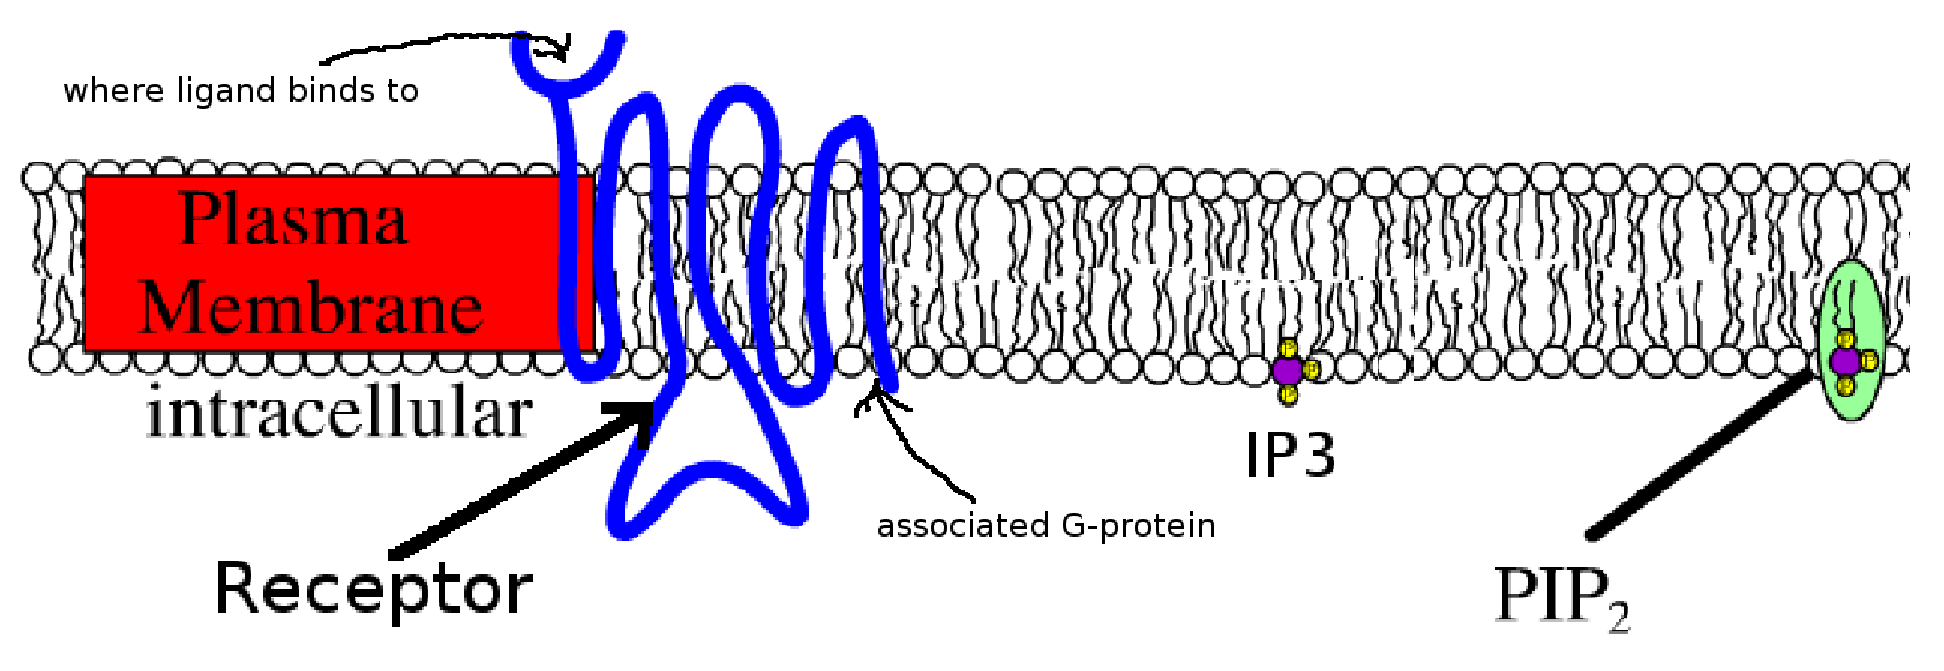
\includegraphics[height=4cm]{./images/IP3.eps}}
\caption{IP3 in the plasma membrane}
\label{fig:IP3}
\end{figure}

 
% Among the many types of G protein-coupled receptors (GPCR -
% Sect.\ref{sec:G-protein-coupled-receptor}), the one with $\alpha$-subunit as
% G$_{q}$ or G$_{11}$, i.e. $G_{\alpha q/11}$ can indirectly trigger the release
% of IP3\footnote{\url{http://en.wikipedia.org/wiki/G_proteins}}.
% 
% Thus, we mainly
% focus on $G_{\alpha q/11}$ subunit.




\subsection{IP3 concentration}
\label{sec:IP3-concentration}

The concentration of Ins(1,4,5)P3 (Sect.\ref{sec:IP3}) in the cell is regulated
by three signaling enzymes: phospholipase C isoforms release Ins(1,4,5)P3 from
the plasma membrane by hydrolysis of PIP2 (Sect.\ref{sec:PIP2}), whereas
inositol phosphate 5-phosphatases remove IP3 by dephosphorylation and a group of
inositol phosphate kinases eliminate it by further phosphorylation at its 3- or
6-hydroxy group (Sect.\ref{sec:IP3-degradation}).
\begin{verbatim}
IP3 = 1,3,5-triphosphatse

(1) dominate at low IP3
IP3 ---[3-Kinase]--> IP4 --[5-phosphastase]--> 1,3,4-triphosphase (I-1,3,4-P3)

(2) dominate at high IP3
IP3 ---[5-phosphatase]--> IP2 --> IP1 --> I
\end{verbatim}

The measured dissociation constant for IP3 and the IP3 receptor/channel ranges
from 1nM to 100 nM depending on the receptor isotype, tissue, and
experimental conditions.
The binding sites or states involved in physiologic Ca21 signaling are not
known due to obscure basal level of IP3.

Since the IP3 receptor in Xenopus oocytes is nearly identical to the type I
receptor of mammalian cells, the range of [IP3] in most mammalian cells is
likely to be similar to that in the oocyte. The choice of the value is important
as it determines the fraction of IP3R opening at rest
(Sect.\ref{sec:IP3-affinity-IP3R}).

\begin{enumerate}
  \item Xenopus oocyte :

Luzzi et al. (1998) found basal IP3 level is \textcolor{red}{40$\pm$10 nM}.
After applying LDA to activate GPCR (producing IP3) for 2 min, peak IP3 level
increased to 650 nM; with maximum peak was 1.8 $\muM$. It is thus suggested
under these conditions, the physiologic range of [IP3] was from 40 nM to 2
$\muM$.

  
  \item HELA cells: 
  
  \item Atrial myocyte: 
  In cultured neonatal cardiac myocytes, using FIRE-1 sensor, under agonists
  (endothelin-1, phenylphrine, angiotensin II), the peak free IP3 was estimated
  30 nM \citep{remus2006ip3con}. Then, the basal value of
  IP3 was testimated 15 nM \citep{cooling2007mhip3}.

% Modeling studies in atrial myocytes estimated the basal value is \~{} $15 nM$,
% increases to maximal value is \~{} $35 nM$ within \~{} $400s$, and then declines
% to basal values within tens of minutes\citep{cooling2007mhip3}.
% Upon stimulation, intracellular [IP3] may increase by a factor $>12$. Under the
% stimulation of $\alpha$-adrenergic and ET-1, free IP3 increases to \~{} $30
% nM$\citep{remus2006ip3con}. 

   \item 
\end{enumerate}

\subsection{IP3 sensor}
\label{sec:IP3-sensor}

Fluorescent IP3 sensors based on the IP3 binding domain of IP3R have recently
been developed (Tanimura et al., 2004; Sato et al., 2005; Remus et al., 2006)
\begin{enumerate}
  \item FIRE (Fluorescent IP3-responsive element) by using IP3-binding domain
  of IP3 isoforms 1, 2, and 3.  \citep{remus2006ip3con}

FIRE-1 for IP3R-1, and showed $K_d = 31.3 \pm 6.7$ nM IP3.
 
  \item IRIS (IP3R-based IP3 sensor) (Matsuura, Mikoshiba, 2006)

IRIS-1 for IP3R-1, and showed $K_d = 549 \pm 62$ nM IP3; is significantly lower
than those of fusion proteins composed of residues 224-604 (Kd = 107 $\pm$ 41 nM; n
= 3), 224-584 (Kd = 105 $\pm$ 0 nM; n = 3), and 224-579 (Kd = 95 $\pm$ 38 nM). 

On Sf9 cells, IP3-sensitivity with Kd = 437$\pm$30 nM; slightly higher than the
value (above) measured in COS7 cell.

\end{enumerate}


\section{-- IP3R in cardiac cells}
\label{sec:IP3R_cardiac}
\label{sec:IP3R-heart}

% In the scale of this book, we will cover the role of IP3 in cardiomyocytes whose
% most obvious function is to contract rhythmically and in a controlled manner.

The notion that IP3 mediates $\Ca$ release from ER/SR in the heart is not new.
However, due to the overwhelm of $\Ca$ from RyRs, IP3Rs have been largely
overlooked, and often regard as making a minor contribution, if any, to
 $\Ca$ signaling.
Recently, the role of IP3 in normal function of the heart has been raised
\citep{hund2008} (Sect.\ref{sec:IP3R_cardiac}).

Currently, it is not known well whether IP3 generation is just a vestigial
pathway or indeed plays an active role in cardiac signalling. No matter what its
function is, there is strong evidence that there is no substantial role for IP3
and its associated \ce{Ca^2+} release in normal EC
coupling\citep{woodcock2005ip3}.


Although published data have suggested that all IP3R isoforms are
expressed in cardiac myocytes, the majority of recent reports concur
that Type 2 IP3R constitutes the predominant channel
isoform~\citep{li2005et1} (Sect.\ref{sec:IP3R-2}). 

In heart, IP3R1 could be involve in physiological modulation of cardiac
contractility, but does NOT play any major role in EC coupling in either cardiac
or skeletal muscle\footnote{Kinetics of \ce{Ca^2+} release from IP3R1 is too
slow compare with Type 2 RyRs to contribute to \ce{Ca^2+} transient during EC
coupling}.
In addition, with its presence in the intercalated discs, it suggests a role in
cell-cell communications and its presence at high level in Purkinje fibers, it
suggests a role in generating cardiac rhythms.

Interestingly, the role of IP3R-dependent \ce{Ca^2+} release appear to be
species-dependent\citep{domeier2007ird}. Thus, we will describe IP3R2 and IP3R3
based on species.

\begin{itemize}
\item In rabbit: IP3R2 and IP3R3 are expressed in both atrial and
  ventricular myocytes\citep{domeier2007ird}.  in rabbit, the
  expression of each type in atrial myocytes is 3- to 4-fold higher
  than that in ventricular myocytes while the expressions of RyRs was
  similar between the two tissues, as shown in
  Fig.~\ref{fig:RyR_IP3R_expression}

\item In rat: IP3R2 and IP3R3 are expressed in both atrial and
  ventricular myocytes. The ratio of IP3R in atrial to ventricular is
  $\tilde 6-fold$)\citep{lipp2000fip3}.

\item In guinea pig: 

\item In human:

\end{itemize}


\subsection{cardiac development}
\label{sec:cardiac-development}

The determination of which types of \ce{Ca^2+} release channels are
present at each of the major stages of murine development provides the
basis for further understanding of how \ce{Ca^2+}-dependent signaling
plays a role in growth and development.  Studies in pre-natal cardiac
and embryonic stem cell-derived myocytes
\footnote{stem cell-derived myocytes grown {\it in vitro} can
  recapitulate the development and differentiation of cardiac cells
  very closely}
have indicated that IP3Rs may play a significant role in cardiac
development, and initiation of pacemaker activity. 

Takeshima et al.'s study on young embryonic rat heart cells showed
that RyR2 deactivation at embryonic day (E) 10 causes major cardiac
defects. However, it was normal with \ce{Ca^2+} release from
intracellular stores at embryonic day
E7.5-9.5~\citep{takeshima1998ela}.  IP3Rs are expressed very early
(E5.5) while RyRs are not abundant until E8.5 or
later~\citep{rosemblit1999icr}.  IP3Rs' expression declines as the
cells differentiate and other \ce{Ca^2+}-handling are put into place.
These data indicate that IP3Rs expressed earlier than RyRs in the
developing heart 


The above results, as well as other evidences, suggest that IP3Rs may
be responsible for the early cycling of \ce{Ca^2+} in developing
myocytes prior to the maturation of EC
coupling~\citep{kockskamper2008ip3}.  The \ce{Ca^2+} cycling within the
developing heart switches from reliance on IP3R to pacemaker currents,
voltage-gated \ce{Ca^2+} and RyRs. However, IP3Rs are not entirely
lost during fetal development. It continues to demonstrate in neonatal
animals, and in adulthood.


Complete depletion of Type 1, Type 2, or Type 3 IP3Rs in mice, or
combined knockout of Types 2 and 3 does not prevent the normal
development of murine heart (or whole animal). These results could
indicate that either (1) IP3Rs are not essential for cardiogenesis, or
(2) there are some unknown redundancy between IP3R isoforms, such that
the presence of any of the three isoforms will do. 


\subsection{neonatal cells}
\label{sec:neonatal-cells}

Neonatal animals have relatively high expression of IP3R compared to
adult cells, and demonstrate to be of functional. Neonatal cardiac
cells response to different agonists (endothelin-1 (ET-1), angiotensin
II, phenylephrine, ATP, pros-taglandins, IGF-1) for IP3 production and
\ce{Ca^2+} mobilization~\citep{jaconi2000ip3,shubeita1990et1}.
However, these same agonists also promote hypertrophic growth of
neonatal cardiac cells~\citep{shubeita1990et1,iwaki1990aba} IP3R1,
IP3R2, and IP3R3 are all expressed in neonatal
cells\citep{kockskamper2008ip3}.


\subsection{matured cardiac cells}
\label{sec:matur-card-cells}


IP3 is an important activator of a specific class of ER/SR \ce{Ca^2+}
release channels (aka IP3R), while neither Ins(1,3,4,5)P4 nor
Ins(1,4)P2 is an effective ligand at IP3Rs~\citep{wilcox1998ndp}. In
addition, IP3 is unlikely to activate IP3Rs far away form its site of
generation. So, \textcolor{red}{a local control is highly suggested}.
IP3Rs are often localized close to the plasma membrane and upstream
receptor-PLC
complexes\footnote{In neurons, there are 2 different PLC-coupled
  receptors that can produce IP3. However, it's only IP3 produced via
  \ce{B2R}s is able to activate IP3Rs~\citep{delmas2002smd}}.  However,
in atrial myocytes, most IP3Rs are perinuclear. There are evidences
that IP3R present on the plasma membrane of some cell types
also~\citep{vazquez2002ip3r}. IP3R are regulated by \ce{Ca^2+} and IP3,
and are modulated by many additional signals.

IP3/IP3R-dependent \ce{Ca^2+} release in cardiac tissues was
demonstrated since early 1980s~\citep{hirata1984rci,nosek1986ite}.
Recently, there are evidence to show IP3-induced \ce{Ca^2+} release
from other microdomains, e.g. Golgi, nuclear
envelope~\citep{rizzuto2006mic}.  Even though, IP3R-dependent
\ce{Ca^2+} release represents the main avenue of intracellular
\ce{Ca^2+} release in electrically non-excitable cells; in excitable
cells, especially cardiac myocytes, the main pathways occur through
RyRs (about 100-fold).
\textcolor{red}{ \ce{Ca^2+} release from a single IP3R is called
  \ce{Ca^2+} blips; while \ce{Ca^2+} release from a cluster of IP3Rs
  is termed \ce{Ca^2+} puffs.}
In comparison to \ce{Ca^2+} sparks, \ce{Ca^2+} puffs has amplitudes
which were 75-80\% smaller, while were about 3 times longer-lasting,
and their rise time was prolonged approximately
two-fold~\citep{kockskamper2008ip3}.

So far, the understanding of the functions of
\hyperref[sec:ip3-pathways]{\it IP3-signaling pathways} is far from
complete.  For a better understanding of IP3 and IP3R's functions,
it's important to know the temporal-spatial localization of IP3
generation, and IP3R, as well as the mechanism of how IP3 induces the
release of \ce{Ca^2+} and how it affects to the release.
\textcolor{red}{We'll focus those properties on cardiac myocytes of
  different species. Further, only IP3R2 and IP3R3 are of mainly
  interest.}

% IP3/IP3R-dependent \ce{Ca^2+} release in cardiac tissues was
% demonstrated since early 1980s~\citep{hirata1984rci,nosek1986ite}. On
% average, IP3R release approximately 30-50\% of the calcium taken up by
% the non-mitochondrial pool of calcium, the remainder can be released
% by calcium ionophores.


\ce{Ca^2+} signaling in cardiac myocytes is composed of not only
global \ce{Ca^2+} signals, but also of spatially restricted \ce{Ca^2+}
signals within signaling {\it microdomains}.  Accordingly,
IP3R-dependent \ce{Ca^2+} release may not contribute much to global
\ce{Ca^2+} release, yet it may regulate a variety of cellular
processes by altering microdomain $[\ce{Ca^2+}]$. By this way, a
rather straightforward way so that IP3R-dependent \ce{Ca^2+} release
may modulate EC coupling is to increase microdomain [\ce{Ca^2+}] in
the vicinity of RyR release clusters (ultimately, increase sensitivity
of RyR to CICR, and efficiency of EC coupling).
\textcolor{red}{In cat, \ce{Ca^2+}
  ``puffs''\footnote{\ce{Ca^2+} release event through
    a cluster of IP3Rs~\citep{yao1995qpi}} was observed}
  \footnote{tetracaine is RyR2 inhibitor, used to block $\Ca$ release via
  RyR2}~\citep{zima2004ip3}.
\ce{Ca^2+} ``puffs'', however, was not observed in rabbit ventricular
myocytes.  Probably IP3R-mediated \ce{Ca^2+} release in these cells is
below the detection threshold of the confocal microscopy being used.


% As IP3Rs are highly sensitized by an increase in IP3, IP3Rs are often
% localized close to the plasma membrane and upstream receptor-PLC
% complexes.  IP3 regulates many cellular processes to response to many
% stimuli (neurotransmitters, hormones, growth factors).  Several
% studies also have implicated IP3 generation in both
% {\it arrhythmogenic} and {\it hypertrophic responses}.

\begin{figure}[hbt]
  \centerline{\includegraphics[height=4cm]{./images/RyR_IP3R_expression.eps}}
\caption{RyR and IP3R(2,3) expression in atrial and ventricular
  myocytes ($n=4$). Data in (B) are normalized and are shown as $means\pm
  SE$. Significant difference from ventricular myocytes, P<0.05}
\label{fig:RyR_IP3R_expression}
\end{figure}

To see how IP3R mediate SR \ce{Ca^2+} release during EC coupling, the
frequencies and amplitudes of \ce{Ca^2+}
sparks\footnote{\ce{Ca^2+} spark frequency is quantified as number of
  sparks per second within 100$\mu m$ of scanned distance [sparks$\dot
  (100\mu m)^{-1}\dot s^{-1}$
\break
Fluo-4 fluorescence emission (F) as normalized to baseline
fluorescence emission (F$_0$). Changes of intracellular [\ce{Ca^2+}]
are presented as changes of ratio $\Delta F/F_0$ (with $\Delta F = F-F_0$)}
in ventricular myocytes were measured between under control condition
and under the addition of IP3, as shown in
Fig.~\ref{fig:IP3_Ca_spark}. With the addition of IP3, the frequency
of \ce{Ca^2+} increase (after 1min); thus cause a reduction of SR
\ce{Ca^2+} content. As a result, it causes a feedback on SR \ce{Ca^2+}
release, i.e. \ce{Ca^2+} spark frequency decrease (after 5min) and the
amplitudes decrease.

\begin{figure}[hbt]
 \centerline{\includegraphics[height=4cm]{./images/IP3_Ca_spark.eps}}
 \caption{(A) \ce{Ca^2+} sparks under control condition (left), 1min
   (center) and 5min (right) after addition of 10$\mu M$ IP3, the
   profile of \ce{Ca^2+} sparks at the bottom correspond to the
   vertical line denoted by black bars at left. (B) The frequency and
   amplitude of \ce{Ca^2+} sparks. Data are normalized to mean of
   values preceding IP3 addition ($t=-4min$ to $t-0$). Significant
   difference from mean value before IP3 addition, $P<0.05$.}
\label{fig:IP3_Ca_spark}
\end{figure}


{\bf Description of Fig.~\ref{fig:IP3_Ca_spark}}: Under control
condition: \ce{Ca^2+} frequency is $17.1\pm 2.0$ sparks $\times$
$(100\mu m)^{-1}\times s^{-1}$ (n=9). With the addition of IP3 ($10\mu
M$): (after 1min) frequency is $121\pm 4.0\%$, n=9 and then return to
baseline after 5-10min; then (after 7min) the amplitude of \ce{Ca^2+}
decreases to $86.9\pm 3.9\%$ of control, n=9, $P<0.05$.
Data are compared using paired or unpaired Student's t-test from $n$
individual cells.


\begin{figure}[hbt]
 \centerline{\includegraphics[height=5cm]{./images/IP3_RyR_relation.eps}}
 \caption{IP3 does not affect RyRs. (A)(B) the incorporation of RyR
   into lipid bilayers does not change; (C) average open probability
   of RyR are similar}
\label{fig:IP3_RyR}
\end{figure}

One experiment has shown that IP3 has no direct effect on RyR
properties, as shown in Fig.~\ref{fig:IP3_RyR}. This was done by
exposing RyR to IP3 by allowing RyR incorporated to the
biomembrane\citep{domeier2007ird}. Another experiment suggested that
effects of IP3 are independent of baseline spark frequency
\citep{domeier2007ird}. At different values of internal [\ce{Ca^2+}]
(150nM, and 100nM), IP3 causes a similar increase in \ce{Ca^2+} spark
frequency (to $124\pm 3\%$ of control).  Another experiment shown that
effect of IP3 on RyR-mediated \ce{Ca^2+} release was IP3R
dependent. This was done by deactivate IP3R using an IP3R
antagonist\footnote{2-aminoethoxydiphenylborate = 2-APB, 20$\mu M$, or
  heparin (HEP), 0.5mg/ml},
and IP3 then has no effect on \ce{Ca^2+} spark frequency, as shown in
Fig.~\ref{fig:IP3_RyR_effect} \citep{domeier2007ird}.  Further, the
effect of endothelin (ET-1) has been shown to induced near-maximal IP3
production\footnote{however, it's not ET-1 alone but with numerous
  cellular targets being implicated in the
  response\citep{domeier2007ird}}, and increase fractional SR
\ce{Ca^2+} release via IP3R activation, independent of total
\ce{Ca^2+} content. Further, ET-1 produced biphasic nagative and
positive inotropic effects on the amplitude of \ce{Ca^2+} transient,
i.e. a brief initial inhibition followed by a secondary increase that
reached maximum after 15min.

\begin{figure}[hbt]
 \centerline{\includegraphics[height=5cm]{./images/IP3_RyR.eps}}
\caption{IP3 does not effect on RyRs. By deactivating IP3R using
  antagonist(2-APB, and HEP), the increase in \ce{Ca^2+} frequency is
  not significant }
\label{fig:IP3_RyR_effect}
\end{figure}

% . The activation of cell
% surface receptors caused small, localized change in [\ce{Ca^2+}]
% adjacent to the plasma membrane. However, such \ce{Ca^2+} signals do
% not induce a perinuclear response
% {\bf NOTE}:
% \textcolor{red}{In neurons, there are 2 different PLC-coupled
%   receptors that can produce IP3. However, it's only IP3 produced via
%   \ce{B2R}s is able to activate IP3Rs}\citep{delmas2002smd}.


\begin{figure}[htb]
    \centerline{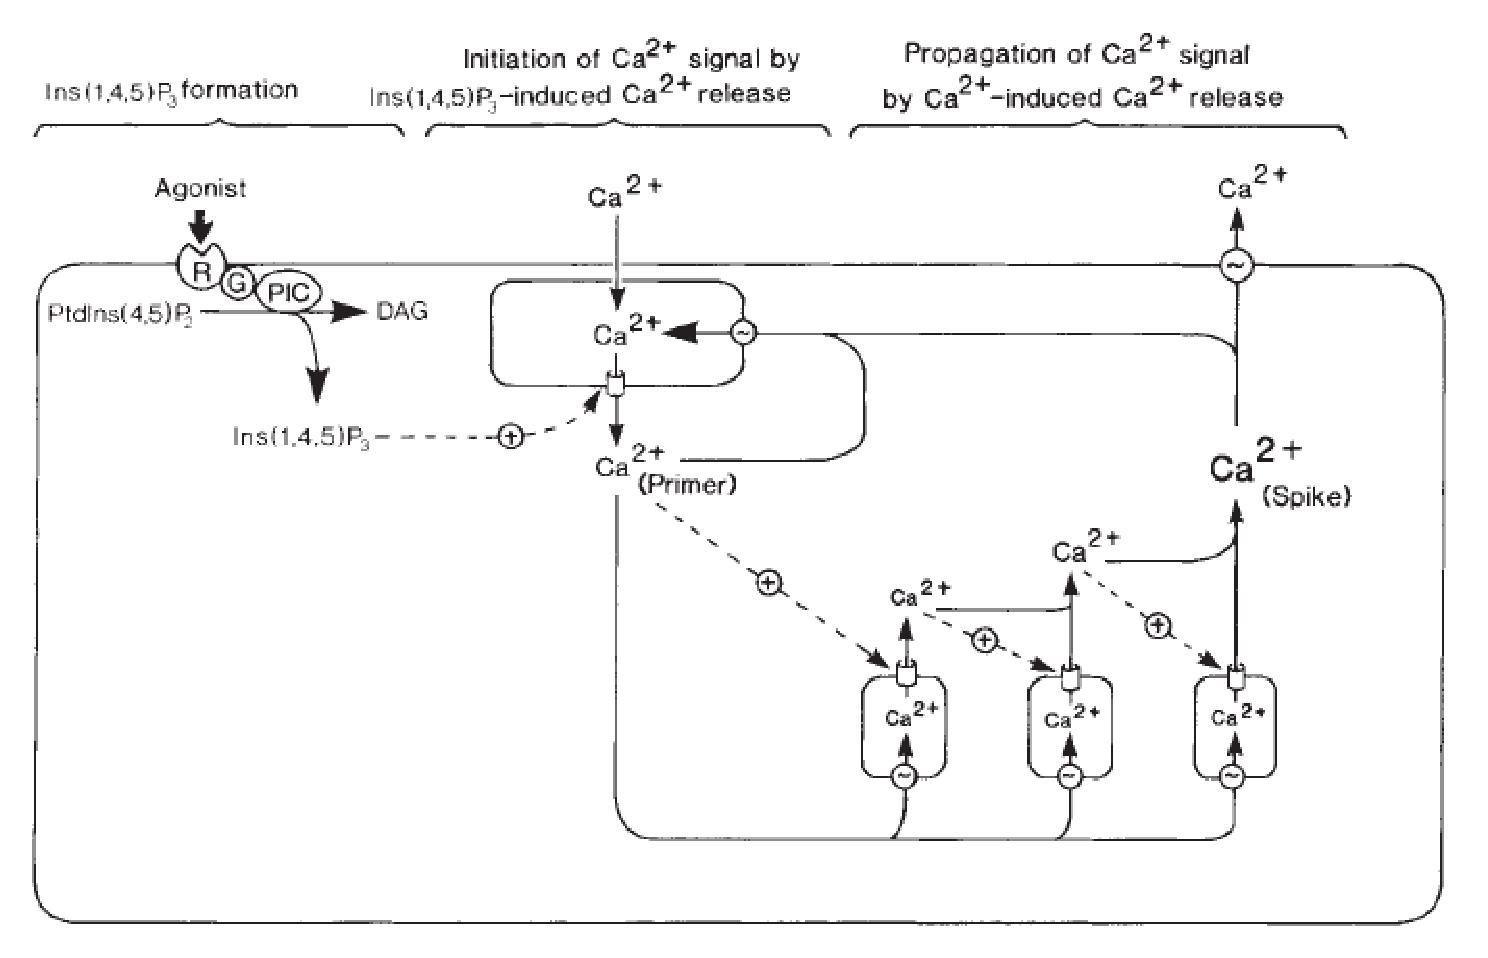
\includegraphics[height=6cm]{./images/IP3_calcium_signalling.eps}}
\caption{A unified hypothesis of the spatio-temporal aspects of
  calcium signalling~\citep{berridge1989ipa}}\label{fig:IP3_Ca_signal}
  \end{figure}
  The mechanism that IP3 control calcium concentration is given in
  Fig.~\ref{fig:IP3_hypothesis}.


\begin{figure}[htb]
    \centerline{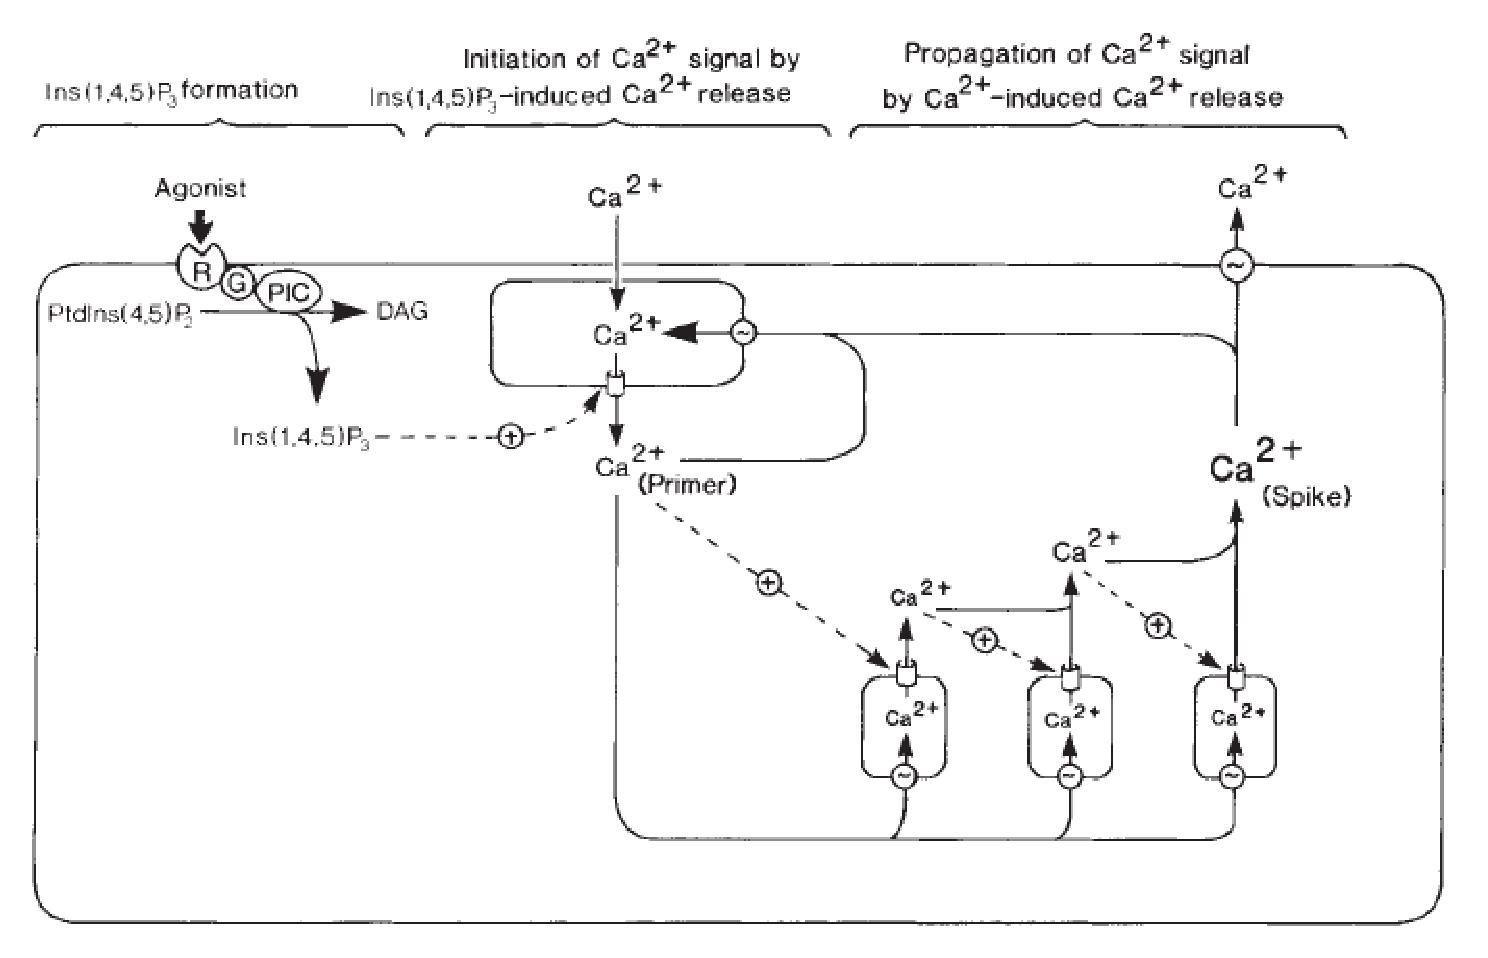
\includegraphics[height=6cm]{./images/IP3_calcium_signalling.eps}}
\caption{A Summary of the proposed mechanism: (a) IP3 control calcium
  channels in the plasma membrane, (B), IP3 control a channel in SR
  which indirectly regulate calcium entry across the biomembrane via a
  {\it negative-feedback loop}; (C) extension of Putney's capacitive
  model - IP3 control the transfer of \ce{Ca^2+} between pools~\citep{berridge1989ipa}}\label{fig:IP3_hypothesis}
  \end{figure}

%How IP3 is metabolized?
% list of enzymes that metabolise IP3


%IP3's receptor

IP3-induced release of calcium showed a steep dose-response
relationship\footnote{dose:concentration of IP3, response:release of
\ce{Ca^2+}} with a clear effect at a concentrations as low as
$0.2\mu$M and a near-maximum release at $5\mu$M ($4.3\pm s.e. 0.5$ nmol
per mg protein, $n=16$).

The calcium-releasing activity depends on the distribution of
phosphates on the inositol ring.  \ce{Ca^2+} was taken up both by
mitochondria and by at least one nonmitochondrial ATP-dependent
\ce{Ca^2+} store. Inhibitors
\begin{itemize}
\item for \ce{Ca^2+} uptake by mitochondria: a combination of the
  mitochondrial inhibitors antimycin A ($10\mu$mol/l) and oligomycin
  ($5\mu$mol/l)
\item for nonmitochondrial \ce{Ca^2+} uptake: completely inhibited
  by high concentrations of the ATPase inhibitor vanadate ($2$ mmol/l) 
\end{itemize}

Experimental results showed that mitochondrial inhibitors do not
impair the ability of IP3 to release \ce{Ca^2+}. This strongly
suggests that IP3 does not release \ce{Ca^2+} from mitochondria. 



{\bf Hypothesis}:  IP3R-dependent \ce{Ca^2+} signaling facilitates
SR \ce{Ca^2+} release during EC coupling in rabbit ventricular
myocytes.




\section{-- IP3R in neurons}
\label{sec:IP3R_neuron}

The neuronal isoform of IP3R is IP3R1, Fig.\ref{fig:IP3R_typeI}
(Sect.\ref{sec:types_IP3R}). IP3R exists a similar supramolecular signaling
complex PP1, PP2A, and PKA like RyR2 (Sect.\ref{sec:RyR_phosphorylation}).

AKAP9 (yotiao) anchoring protein recruits both PKA and PP1 to IP3R1, wherease
PP2A can assemble into the complex through AKAP450 - a longer splice variant of
AKAP9/yotiao.



\section{IP3-Receptors (IP3R)}
%\label{sec:receptors}
\label{sec:IP3R}

The first IP3R was characterized in 1979 as a protein called {\bf
$P_{400}$}\citep{mikoshiba1979bai} (Purkinjie cell-enriched protein of 250 kDa).
Other groups named it as {\bf GP-A}~\citep{groswald1984ece} (a 240 kDa
glycoprotein) and {\bf PCPP-260}~\citep{walaas1986pcpp}; and this IP3R is found
only in SR.


\subsection{Structure and sequences}
%\label{sec:structure-3} 
\label{sec:IP3R-structure}

IP3-receptor was first cloned from cerebellum \citep{furuichi1989}
(Sect.\ref{sec:IP3R_neuron}).

Structurally, IP3R is a large ($\approx 30nm$ in diameter) homomeric tetramer of
four subunits of the same type forming a single ion-conducting
channel~\citep{taylor2004ip3, bezprozvanny2005ip3r}.
Each IP3R subunit has six transmembrane region in the ER.

IP3Rs are structurally and functionally similar to RyRs.
As showed below, the primary sequence of IP3-receptor share no homology with the
\ce{Ca^2+}-channels in the plasma membrane, but shares significant partial
homology with the RyR of the SR in skeletal and cardiac muscles.

There are 3 main forms of IP3R subunits (type 1, 2, 3) have been characterized
by cDNA cloning \citep{patel1999}, as shown in Fig.~\ref{fig:IP3R_topo}, with
molecular mass about 260 kDa (Sect.\ref{sec:types_IP3R}). The three isoforms
have subtly divergent properties \citep{miyakawa1999}.
\begin{itemize}
  \item  IP3R2 share 69\% identity with amino acid sequence of IP3R1. 
  
  \item IP3R3 share 64\% identity with IP3R1~\citep{rosemblit1999icr}. 
  
\end{itemize}

% IP3R is a glycoprotein ; formed by 4 subunits.



% There is not a single IP3-receptor, in fact there are different types.
% \begin{enumerate}
% \item {\bf bradykinin and neurokinin A receptors}: give large rapid
%   \ce{Ca^2+} transients

% \item {\bf lysophosphatidic acid (LPA), thrombin and histamine
%     receptors}: release \ce{Ca^2+} slowly but persist for much longer.
% \end{enumerate}

\begin{figure}[hbt]
 \centerline{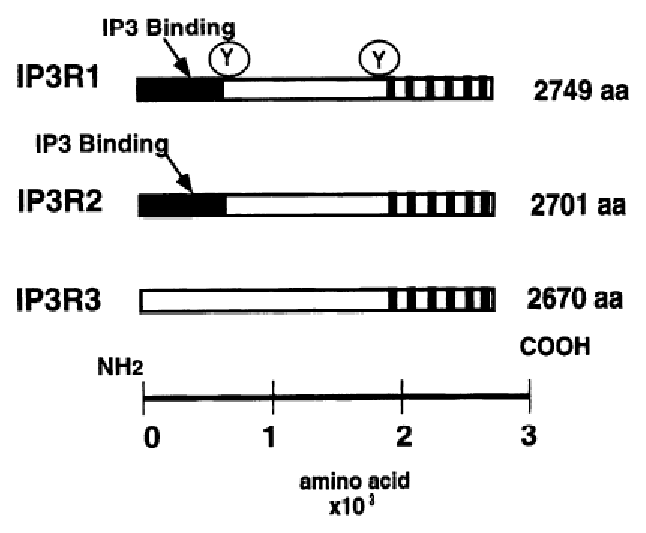
\includegraphics[height=5cm]{./images/IP3R_topography.eps}}
 \caption{The topography of IP3R (1, 2 and 3). Only in IP3R1 and IP3R2
   has IP3 binding sites near the amino terminus. Y is the location of
 putative tyrosine phosphorylation site}
 \label{fig:IP3R_topo}
\end{figure}


\begin{figure}[htb]
  \centerline{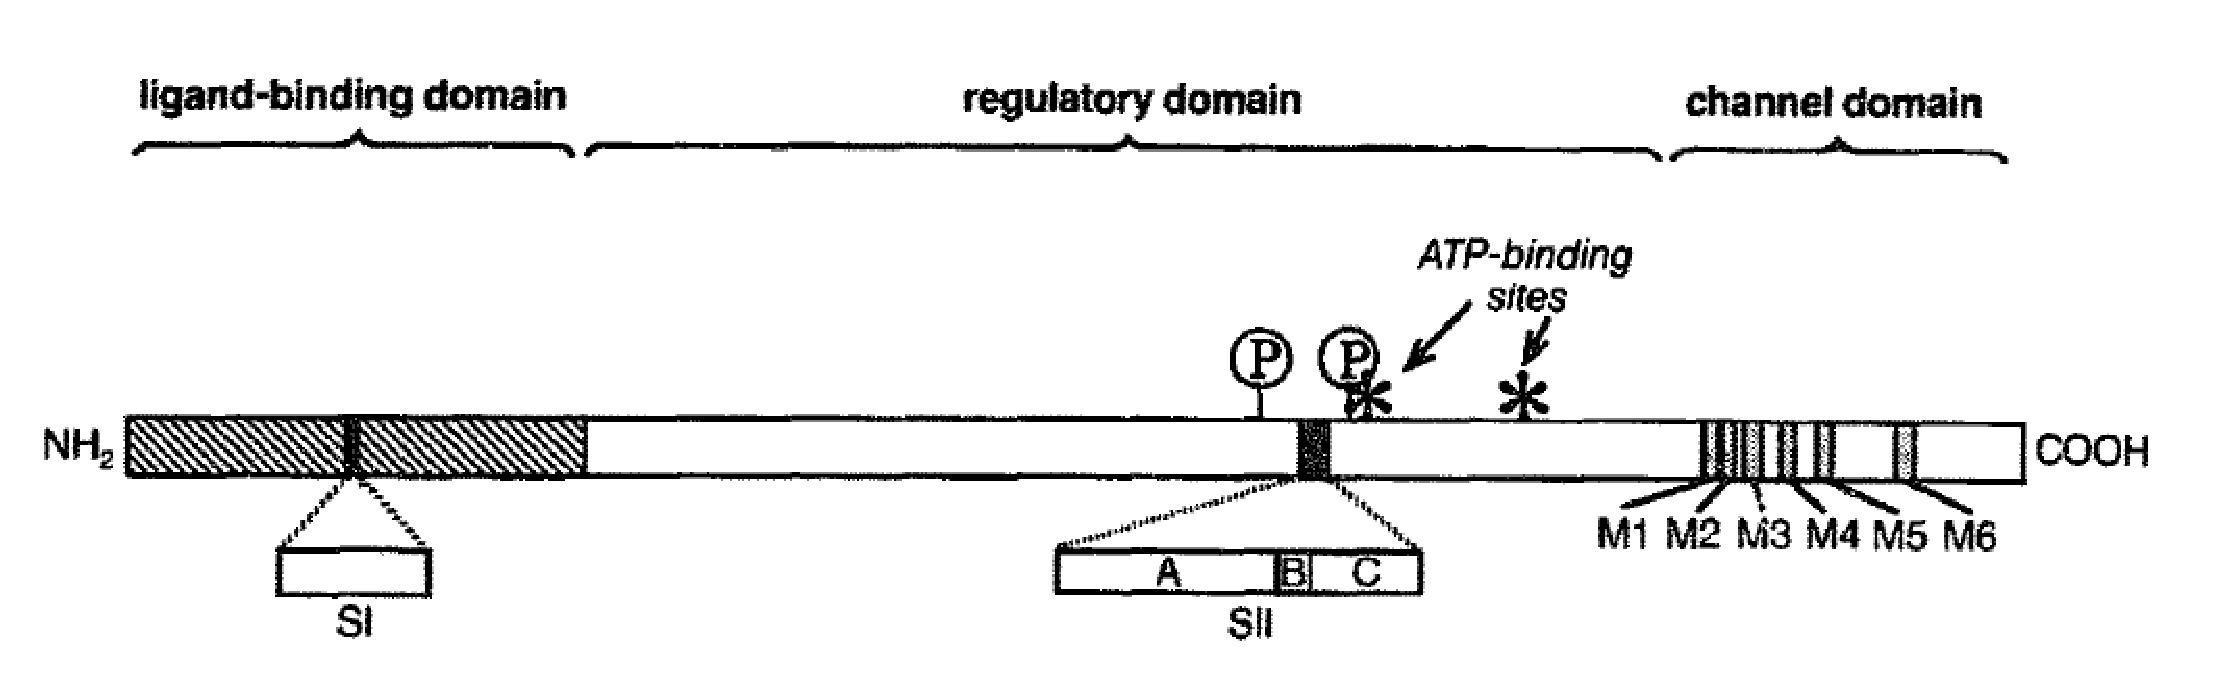
\includegraphics[height=4cm]{./images/IP3-receptor_sequence.eps}}
  \caption{Amino Acid Sequence of IP3-receptor type 1}\label{fig:IP3-receptor_seq}
\end{figure}

\begin{figure}[htb]
  \centerline{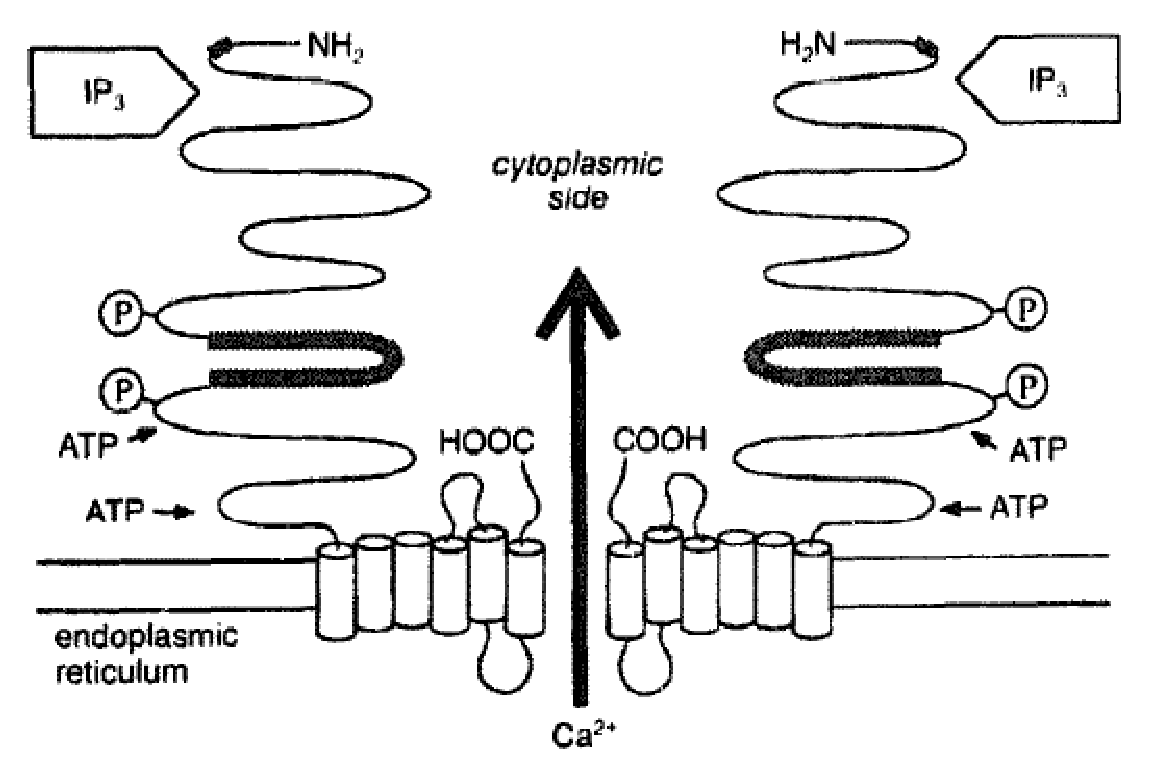
\includegraphics[height=6cm]{./images/IP3-receptor_subunit_pore.eps}}
  \caption{A diagram of an IP3-receptor in ER}
  \label{fig:IP3-receptor_pore}
\end{figure}



Most cells have at least one type of IP3R, and many express all three
types.  Cloning the cDNA of the IP3-receptor in mouse showed its amino
acid sequence, as shown in Fig.~\ref{fig:IP3-receptor_seq}, with 3
functionally different domains: ligand (IP3)-binding domain,
regulatory domain, and channel domain~\citep{mikoshiba1993itr}.


\begin{itemize}
\item P: phosphorylation sites

\item SI, SII: isoforms produced by alternate RNA splicing

\item M1-M6: 6 membrane-spanning regions near the C-terminus
\end{itemize}
The channel can be devided into 3 regions: N-terminal ligand-binding domain,
central regulatory domain, and C-terminal channel domain,
Fig.\ref{fig:IP3R_typeI}. As shown in Fig. \ref{fig:IP3-receptor_seq} and
\ref{fig:IP3-receptor_pore}, an IP3R subunit has a long N-terminus and
a short C-terminus outward to the cytoplasm.  As shown here, the first
650 N-terminal residues is mainly function as IP3-binding sites. 

The specific high-affinity binding site for IP3 was first identified in bovine
adrenal cortex \citep{baukal1985}. Amino acids from 224-538 are the minimal
sequence sufficient for IP3-binding \citep{yoshikawa1996}. However, it's more
likely IP3-binding site is composed of multiple sequences scatterred within the
N-terminal region of the protein \citep{patel1999}.

% IP3Rs form \ce{Ca^2+}-channels and are
% activated by IP3 synthesized from $G_{\alpha q/11}$ , ATP and
% \ce{Ca^2+}. 



\subsection{Classification (isoforms)}
\label{sec:classification}
\label{sec:types_IP3R}

IP3Rs channel are classified based on the type of IP3R subunits. Thus,
there are also 3 types of IP3-receptors. 
The two additional isoforms: IV and V are proposed to exist, based on partial
sequence information \citep{ross1992,de_smedt1994}.

Type II IP3R has been suggested to undergo
alternative splicing \citep{sudhof1991}; and type IV IP3R can be a splice
variant of type II \citep{ross1992, parys1995}.

\subsection{-- IP3R type 1}
\label{sec:IP3R-type1}

The first discovered IP3R channel is given the name type I (IP3R1). IP3R1 is
regulated by at least two major cellular signalling pathways: IP3 (activate the
channel), nonreceptor protein tyrosine kinases (e.g. Fyn) (increase the open
probability by phosphorylation the IP3R1).  

IP3R1 is the predominant intracellular \ce{Ca^2+}-release channel in vascular
smooth muscle, cerebellum, and human T cells.
IP3R1 express in both human atrial (Sect.\ref{sec:IP3R-heart}) and central
nervous system, i.e. rat Purkinje myocytes\citep{nakanishi1991ip3r,
gorza1993ip3r,yamada2002ip3r}. Type I and III \tIPthreeR isoforms are also found
in Purkinje fibers \citep{bezprozvanny1991ip3r,li2005}, and neonatal
\citep{luo2008}.

\subsection{-- IP3R type 2}
\label{sec:IP3R-type2}
\label{sec:IP3R-2}

IP3R2 has a significantly higher affinity for IP3 than does the IP3R1.
{\it Each tissue may contain several different forms of IP3 receptors
coming from different genes or spliced variants from one gene. Each receptor
may has different \ce{Ca^2+}-releasing activity}.
This suggest the multiple pathways in intracellular \ce{Ca^2+} signalling with
different regulatory properties.

IP3R2 and IP3R3 are found in both atrial and ventricular myocytes
from most animal species, with IP3R2 is more predominant.

However, in adult atrial and
ventricular myocytes, type-2 IP3R is the major isoforms\citep{woodcock1998,
li2005, lipp2000}. Nevertheless, the expression level is about 100-fold lower
than RyR2. Thus, calcium flux through IP3R has always been overlooked. Even though, the
physiological role of type-2 IP3R (IP3R-2) in cardiac cells remain elusive, yet
there are many IP3-inducing agonists (angiotensin II, endothelin,
norepinephrine) involving in hypertrophy and heart failure \citep{bare2005}.


{\bf Localization}: IP3R-2 was found localized at the subcellular level to
cardiomyocyte nuclear envelope (NE) \citep{bare2005, janowski2010}. The
separation of IP3R-2 and RyR2 suggested a functional segregation of these
channels, and possibly a unique role of IP3R-2 in regulating nuclear calcium
dynamics. \citep{janowski2010} found that in developing cardiomyocytes,
IP3R-mediated $\Ca$ signal can be significantly large in amplitude and duration
to trigger contraction and affect CICR process.


IP3R-2 was found in association with Ca/Calmodulin-dependent protein kinase
II$\delta$ (CaMKII$\delta$ - the major isoform of CaMKII expressed in
cardiomyocyte) using immunoprecipatation \citep{bare2005}. CaMKII can
phosphorylate IP3R-2 and result on planar lipid bilayers showed a reduction (11
times) in open probability. The hypothesis was that calcium release from IP3R-2
may activate local CaMKII signalling, which may feedback on IP3R-2 function
\citep{bare2005}.



\subsection{-- IP3R type 3}
\label{sec:IP3R-type3}

IP3R2 and IP3R3 are found in both atrial and ventricular myocytes from most
animal species, with IP3R2 is more predominant.

% IP3R-dependent \ce{Ca^2+} release is well established in the atrial
% myocardium (IP3R2 and IP3R3). Recently, both IP3R2 and IP3R3 have been
% found to express also in ventricular myocytes. In
% particular, activation of IP3R facilitates SR \ce{Ca^2+} release
% through RyRs and enhance \ce{Ca^2+} transient during EC
% coupling. However, . This is similar to but
% not as substantial as that observed for IP3Rs in rat ($\tilde
% 6-fold$)\citep{lipp2000fip3}.





\subsection{Regulatory Factors of IP$_3$R}
\label{sec:IP3R-regulatory-factors}

An IP3R channel has the same tetramic pinwheel structure, i.e. with 4 subunits,
each one is regulated by inositol 1,4,5-triphosphate (\IPthree or InsP$_3$) and
$\Ca$ at the cytosolic binding sites.

With 4 subunits per channel, it has been suggested that in order for the
activation of a single IP3-gated channel, it requires 3 to 4 IP3R subunit in a
single channel to be activated, at least in rat basophilic leukemic (RBL) cells
(Meyer, Holowka, Stryer, 1988; Meyer, Wensel, Stryer, 1990).

Each IP3R subunit, in turns, has 3 binding sites: IP3-binding site (IP3
synthesized from $G_{\alpha q/11}$), activation \ce{Ca^2+}-binding site and an
inhibitory \ce{Ca^2+}-binding site. As the result, we have the schematic of the
states of a single IP3R channel subunit as shown in
Fig.~\ref{fig:IP3R_schematic}~\citep{shuai2007kms}. This is a common way being
used to build the computational model for simulation. 

\begin{figure}[hbt]
 \centerline{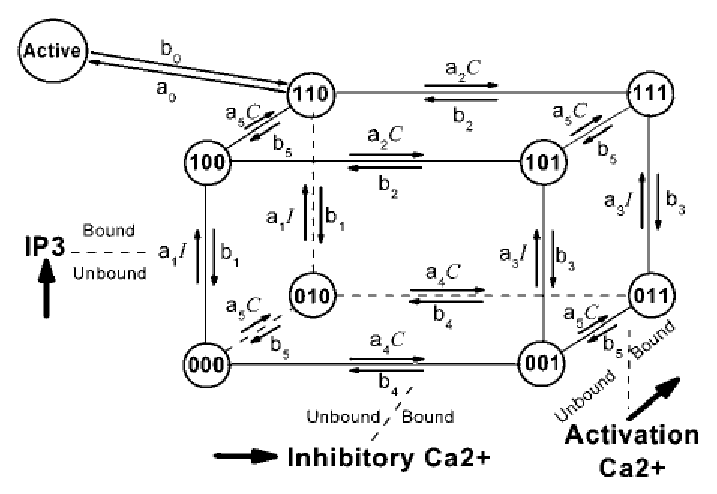
\includegraphics[height=6cm]{./images/IP3R_subunit_schematic.eps}}
 \caption{The schematic diagram of the model of a single IP3R
  subunit. The three binding sites are labeled as ($ijk$) with $i$ index
for IP3-binding site, $j$ is for the activation \ce{Ca^2+}-binding
site, $k$ is for the inhibitory \ce{Ca^2+}-binding site. The number 1
indicate an occupied binding site, and 0 otherwise. The bold arrows
indicates the binding of ligands to different sites}
\label{fig:IP3R_schematic}
\end{figure}

Gating of IP3R is not affected by 2$\muM$ ruthenium red or 5$\muM$ ryanodine.
So it has a different gating mechanism than RyR.

There are different suggested mechanisms, 
\begin{enumerate}
  \item Adenophostin A, the most potent known agonist of inositol
  1,4,5-trisphosphate (InsP3) receptors
  
Compared with IP3: half-maximal effect (EC50 - Sect.\ref{sec:EC50}) for
Adenophostin A is 7.1$\pm$0.5nM, while EC50 for IP3 is 177$\pm$26nM (Adkins et
al., 2000)
  
  \item IP3 binding is precondition:

% So, it can be inferred that the binding of IP3 is a precondition for the
% activation of IP3R. 
 
 \begin{itemize}
   \item cooperative activation by \IPthree (e.g. the opening of an IP3R in rat
  basophilic leukemia cells requires the binding of at leat 3 \IPthree
  \citep{meyer1988})
  \end{itemize}
  
  
  \item Multiple binding sites for $\Ca$ ions: one activation site and one
  inactivation site givine  biphasic feedback of $\Ca$ ions
  \citep{bezprozvanny1991ip3r}
  
IP3R type 1: \citep{sienaert1996,sienaert1997}

Thus, IP3R is regulated by cytosolic $\Ca$, in a biphasic manner
\citep{iino1992}. 

EVIDENCE: \tIPthreeR release $\Ca$ from endoplasmic reticulum (ER)
under the binding of $\Ca$ (to the activation site) and IP$_3$ to the
channel (to decrease the $\Ca$ affinity of the $\Ca$-inactivation site)
\citep{berridge1993, taylor2004, bezprozvanny2005ip3r, foskett2007ip3r}.
Nevertheless, the fully IP3-bounded channels can also be inhibited by $\Ca$,
albeit at sufficiently high $[\Ca]$ \citep{mak2001}.

  \item  The channel also undergo phosphorylation by different protein kinases,
  yet the succeptibility to phosphorylation can be different between IP3R
  isoforms.
  
  \begin{enumerate}
    \item PKA \citep{furuichi1989, joseph1993, wojcikiewicz1998}, 
    
    \item cyclic GMP-dependent protein kinase (PKG)
    \citep{komalavilas1994,koga1994, rooney1996}, 
    
    \item protein kinase C (PKC) \citep{ferris1993,matter1993}, and
    
    \item calmodulin-dependent kinase II (CaMKII) \citep{ferris1993}
  \end{enumerate}
  
  \item AMP-PCP can help to increase IP3R activity:
  
EVIDENCE: When adding AMP-PCP (a poorly hydrolysable analogue of ATP) or $\Ca$
or both, without IP3, the IP3Rs' activity was not observed~\cite{bezprozvanny1991ip3r}.
  
\end{enumerate}




\begin{figure}[hbt]
  \centerline{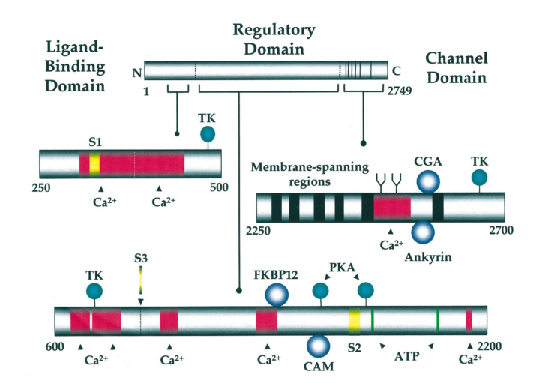
\includegraphics[height=5cm,
    angle=0]{./images/IP3R_type_I.eps}}
\caption{Mouse IP3R type I. The accessory proteins (chromogranin A (CGA),
FK506-binding protein (FKBP12), and calmodulin (CAM)) are depicted as large
blue spheres. Cytosolic phosphorylation sites (for cyclic-AMP-dependent
kinases (PKA), and tyrosine kinases (TK)) are depicted in small green circles.}
\label{fig:IP3R_typeI}
\end{figure}


\subsection{-- IP3-sensitive to IP3R}
\label{sec:IP3-affinity-IP3R}

(1,4,5)IP3 binding was reversibly stimulated by increased pH, i.e. using
competition of $\ce{^3[H]IP3}$.

Nerou et al. (2001), using Sf9 cell, showed that that  6-hydroxy group of
(1,4,5)IP3 was essential for high affinity binding, the equatorial 3-hydroxy group
significantly improved affinity, and the axial 2-hydroxy group was
insignificant.


IP3-affinity by IP3R isoforms are often done using IP3-sensor as competing
binding ligand (Sect.\ref{sec:IP3-sensor}).

Wojcikiewicz and Luo showed that IP3 affinity by IP3R are ranked: IP3R1
$\approx$ IP3R2 > IP3R3. However, this is in contradict to data by Nerou et
al. (2001).

IP3R-type 1: 
\begin{enumerate}
  \item $K_d = 24\pm 4 $nM  (Nerou et al., 2001)
  \item $K_d = 1.5 $ nM (Wilcox et al., 2004)
\end{enumerate}

IP3R-type 2: 
\begin{enumerate}
  \item $K_d = 17\pm 2 $nM (Nerou et al., 2001)
  \item $K_d = 2.5$ nM 
\end{enumerate}

IP3R-type 3: 
\begin{enumerate}
  \item $K_d = 11\pm 2 $nM (Nerou et al., 2001)
  \item $K_d = 22.4$ nM 
\end{enumerate}

\subsection{-- IP3R blockers}
\label{sec:IP3R-blockers}

IP3R antagonists include: 20 $\muM$ 2-APB (2-aminoethoxydiphenyl borate) and
heparin (0.5mg/ml) [Domeier et al., 2008].

\subsection{Subcellular Distribution}
\label{sec:IP3R-distribution}


IP3-R are generally thought to reside in endoplasmic reticulum / sarcoplasmic
reticulum (ER/SR) of almost all cell types with structurally and functionally
distinct from all other ion channels. 

However, in some tissues, IP3-R have been localized to plasma membrane where
they can gate \ce{Ca^2+} influx, e.g. T-lymphocytes \citep{kuno1987, khan1992,
vazquez2002ip3r}, nuclei of liver \citep{nicotera1990}, Xenopus oocyte
\citep{stehno_bittel1994, gerasimenko1995}, cerebellum (where it is present almost entirely in Purkinje
neuron) \citep{joseph1989ip3,joseph1992}.
% IP3Rs is found on endoplasmic reticulum (ERs) of almost all types of cells
\footnote{\url{http://www.bio.davidson.edu/courses/immunology/Flash/IP3.html}}.


Other studies showed IP3R in releasing $\Ca$ from secretory vesicles
\citep{yule1997}, and golgi apparatus \citep{pinton1998}.

In cardiac cells, IP3R type II are found in nucleus envelope
\citep{janowski2010,bare2005}. Immunoblotting of protein from ventricular
myocytes showed expression of both type II and III at level of 3.5-fold less
than atrial myocytes \citep{domeier2008}.



\section{Unresolved questions}
\label{sec:unresolved-questions}

\subsection[Q1]{Why cardiac myocytes express different IP3R isoforms?}
\label{sec:why-cardiac-myocytes}


\subsection[Q2]{What is the composition, subcellular distribution, and functional role of IP3Rs in cardiac cells?}
\label{sec:what-comp-subc}




\subsection[Q3]{How is expression of IP3R regulated?}
\label{sec:how-expression-ip3r}


\subsection[Q4]{What kinases \& phosphatases regular cardiac IP3R phosphorylation}
\label{sec:what-kinases-}


\subsection[Q5]{How exactly is IP3 signaling involving in development and pregression of cardiac diseases?}
\label{sec:how-exactly-ip3}


%%% Local Variables: 
%%% mode: latex
%%% TeX-master: "thermo-stat"
%%% End: 
